\documentclass[conference]{IEEEtran}
\IEEEoverridecommandlockouts
\usepackage{cite}
\usepackage{amsmath,amssymb,amsfonts}
\usepackage{algorithmic}
\usepackage{algorithm}
\usepackage{graphicx}
\usepackage{textcomp}
\usepackage{xcolor}
\usepackage{tikz}
\usepackage{booktabs}
\usepackage{multirow}
\usepackage{array}
\usepackage{colortbl}
\usepackage{hyperref}
\usepackage{subcaption}
\usetikzlibrary{shapes.geometric, arrows, positioning, fit, backgrounds, calc, decorations.pathreplacing, patterns}

\def\BibTeX{{\rm B\kern-.05em{\sc i\kern-.025em b}\kern-.08em
    T\kern-.1667em\lower.7ex\hbox{E}\kern-.125emX}}

% Custom colors
\definecolor{agentblue}{RGB}{70,130,180}
\definecolor{envgreen}{RGB}{60,179,113}
\definecolor{rewardorange}{RGB}{255,140,0}
\definecolor{tablehead}{RGB}{230,230,250}
\definecolor{bestgreen}{RGB}{200,255,200}

% TikZ styles
\tikzstyle{startstop} = [rectangle, rounded corners, minimum width=1.8cm, minimum height=0.6cm, text centered, draw=black, fill=red!20]
\tikzstyle{process} = [rectangle, minimum width=1.8cm, minimum height=0.6cm, text centered, draw=black, fill=blue!15]
\tikzstyle{decision} = [diamond, minimum width=1cm, minimum height=0.5cm, text centered, draw=black, fill=green!15, aspect=2.5]
\tikzstyle{arrow} = [thick,->,>=stealth]
\tikzstyle{io} = [trapezium, trapezium left angle=70, trapezium right angle=110, minimum width=1cm, text centered, draw=black, fill=yellow!20]

\begin{document}

\title{Cloud Auto-scaling using Reinforcement Learning:\\
A Comparative Study of Tabular and Deep RL Methods}

\author{\IEEEauthorblockN{Srivatsa Balasubramanyam}
\IEEEauthorblockA{\textit{Computing id: mhe3sy} \\
\textit{University of Virginia}\\
mhe3sy@virginia.edu}
\and
\IEEEauthorblockN{Ryan Arthur Healy}
\IEEEauthorblockA{\textit{Computing id: rah5ff} \\
\textit{University of Virginia}\\
rah5ff@virginia.edu}
\and
\IEEEauthorblockN{Bruce Mcgregor}
\IEEEauthorblockA{\textit{Computing id: bm3pk} \\
\textit{University of Virginia}\\
bm3pk@virginia.edu}
}

\maketitle

\begin{abstract}
Cloud computing platforms rely heavily on auto-scaling mechanisms to dynamically adjust computational resources in response to varying workload demands. Traditional threshold-based approaches suffer from reactive behavior and poor adaptation to dynamic patterns. This paper presents a comprehensive reinforcement learning (RL) approach to cloud auto-scaling, comparing six algorithms across baseline, tabular RL, and deep RL categories. Our Gymnasium-compatible simulator generates realistic workloads using synthetic patterns combining sinusoidal trends with stochastic spikes. The state representation includes a novel \textit{trend feature} enabling anticipatory scaling. Experiments over 1,000 episodes reveal that \textbf{tabular methods (SARSA, Q-Learning) outperform deep RL variants} by 23\% in mean reward, achieving 77\% improvement over random baselines. This counterintuitive finding suggests that for auto-scaling problems with naturally discrete, low-dimensional state spaces ($|S|=45$), simpler methods may be preferable. We provide detailed analysis of convergence behavior, reward function design, and practical deployment considerations.
\end{abstract}

\begin{IEEEkeywords}
Cloud Computing, Autoscaling, Reinforcement Learning, SARSA, Q-Learning, DQN, Resource Management, Service Level Agreements
\end{IEEEkeywords}

\section{Introduction}

\subsection{Problem Statement}
Cloud auto-scaling determines \textit{when} and \textit{how much} to adjust computational resources in response to workload changes. The goal is to minimize costs while satisfying Service Level Agreements (SLAs). This sequential decision-making problem under uncertainty is naturally formulated as a Markov Decision Process (MDP).

Traditional threshold-based policies (e.g., ``scale up when CPU $>$ 80\%'') are simple but suffer from:
\begin{itemize}
    \item \textbf{Reactive lag}: Responding only after degradation occurs
    \item \textbf{Parameter sensitivity}: Fixed thresholds fail across workload types
    \item \textbf{No learning}: Cannot improve from experience
\end{itemize}

Reinforcement learning addresses these limitations by learning policies that map states to actions through interaction, potentially discovering proactive strategies.

\subsection{Research Questions}
This work investigates three research questions:
\begin{enumerate}
    \item[\textbf{RQ1}:] Can RL agents learn effective auto-scaling policies that outperform threshold baselines?
    \item[\textbf{RQ2}:] Do deep RL methods provide advantages over tabular methods for auto-scaling?
    \item[\textbf{RQ3}:] What state features enable anticipatory (vs. reactive) scaling behavior?
\end{enumerate}

\subsection{Contributions}
Our contributions are:
\begin{enumerate}
    \item A Gymnasium-compatible auto-scaling simulator with configurable workload patterns and a multi-objective reward function (Section~\ref{sec:environment})
    \item Empirical comparison of six algorithms showing tabular methods outperform deep RL (Section~\ref{sec:results})
    \item Analysis of the \textit{trend feature} for anticipatory scaling (Section~\ref{sec:discussion})
    \item Open-source implementation with reproducible experiments\footnote{Code: \url{https://github.com/rah-ds/Cloud-Autoscaling-using-RL}}
\end{enumerate}

\section{Related Work}

\subsection{Threshold and Rule-Based Approaches}
Commercial cloud platforms (AWS Auto Scaling, Azure VMSS) primarily use threshold-based policies with cooldown periods. While simple, these require manual tuning per workload and cannot optimize multi-objective trade-offs \cite{garcia2020}.

\subsection{Predictive Approaches}
Time-series forecasting (ARIMA, LSTM) can predict future demand, enabling proactive scaling \cite{xu2022}. However, prediction errors compound, and the scaling logic remains static.

\subsection{Reinforcement Learning Approaches}
Recent work applies RL to cloud resource management:
\begin{itemize}
    \item \textbf{AWARE} \cite{qiu2023}: Production RL auto-scaling at scale, highlighting safe exploration challenges
    \item \textbf{DeepRM} \cite{mao2016}: Deep RL for cluster scheduling
    \item \textbf{Decima} \cite{mao2019}: Graph neural networks for job scheduling
\end{itemize}

Our work differs by systematically comparing tabular vs. deep methods and identifying when simpler approaches suffice.

\section{Environment Design}
\label{sec:environment}

\subsection{System Architecture}
Figure~\ref{fig:architecture} shows the RL framework. The agent observes state $s_t$, takes action $a_t$, receives reward $r_t$, and transitions to $s_{t+1}$.

\begin{figure}[htbp]
\centering
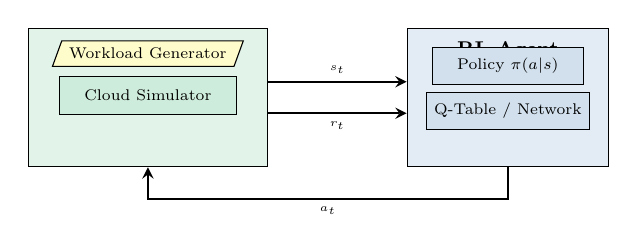
\begin{tikzpicture}[node distance=1.2cm, scale=0.8, transform shape]
    % Environment box
    \node (env) [process, minimum width=3.8cm, minimum height=2.2cm, fill=envgreen!15] {};
    \node at (env.north) [anchor=north, yshift=-0.1cm, font=\small\bfseries] {Environment};
    \node (workload) [io, below=0.2cm of env.north, minimum width=2.8cm, font=\scriptsize] {Workload Generator};
    \node (sim) [process, below=0.15cm of workload, minimum width=2.8cm, fill=envgreen!25, font=\scriptsize] {Cloud Simulator};
    
    % Agent box
    \node (agent) [process, right=2.2cm of env, minimum width=3.2cm, minimum height=2.2cm, fill=agentblue!15] {};
    \node at (agent.north) [anchor=north, yshift=-0.1cm, font=\small\bfseries] {RL Agent};
    \node (policy) [process, below=0.3cm of agent.north, minimum width=2.4cm, fill=agentblue!25, font=\scriptsize] {Policy $\pi(a|s)$};
    \node (value) [process, below=0.1cm of policy, minimum width=2.4cm, fill=agentblue!25, font=\scriptsize] {Q-Table / Network};
    
    % Arrows
    \draw [arrow] ([yshift=0.25cm]env.east) -- node[above, font=\tiny] {$s_t$} ([yshift=0.25cm]agent.west);
    \draw [arrow] ([yshift=-0.25cm]env.east) -- node[below, font=\tiny] {$r_t$} ([yshift=-0.25cm]agent.west);
    \draw [arrow] (agent.south) -- ++(0,-0.5) -| node[below, pos=0.25, font=\tiny] {$a_t$} (env.south);
\end{tikzpicture}
\caption{RL Auto-scaling Framework}
\label{fig:architecture}
\end{figure}

\subsection{MDP Formulation}

\subsubsection{State Space}
We use a discrete state representation enabling tabular methods:
\begin{equation}
s_t = (\underbrace{u_t}_{\text{utilization}}, \underbrace{c_t}_{\text{capacity}}, \underbrace{\tau_t}_{\text{trend}})
\end{equation}

Table~\ref{tab:state} defines each component. The total state space size is $|S| = 3 \times 5 \times 3 = 45$ states.

\begin{table}[htbp]
\centering
\caption{State Space Components}
\label{tab:state}
\begin{tabular}{llll}
\toprule
\textbf{Feature} & \textbf{Symbol} & \textbf{Values} & \textbf{Meaning} \\
\midrule
Utilization & $u_t$ & $\{0,1,2\}$ & Low/Med/High \\
Capacity & $c_t$ & $\{1,...,5\}$ & Active units \\
Trend & $\tau_t$ & $\{-1,0,+1\}$ & $\text{sign}(d_t - d_{t-1})$ \\
\bottomrule
\end{tabular}
\end{table}

The \textbf{trend feature} $\tau_t$ captures demand direction, enabling the agent to learn anticipatory policies (e.g., scale up when demand is rising, even if current utilization is acceptable).

\subsubsection{Action Space}
Three discrete actions:
\begin{equation}
a_t \in \mathcal{A} = \{\text{down}(-1), \text{hold}(0), \text{up}(+1)\}
\end{equation}

Actions are constrained by capacity bounds $[C_{\min}, C_{\max}]$.

\subsubsection{Reward Function}
The reward function encodes multiple objectives. Based on extensive tuning, we use:

\begin{equation}
r_t = r_{\text{util}} + r_{\text{SLA}} + r_{\text{waste}} + r_{\text{cost}} + r_{\text{churn}}
\label{eq:reward}
\end{equation}

\textbf{Component 1 - Utilization Reward} (target band incentive):
\begin{equation}
r_{\text{util}} = \begin{cases}
+10 & \text{if } 0.40 \leq u_t \leq 0.80 \\
+5 & \text{if additionally } 0.60 \leq u_t \leq 0.70 \\
0 & \text{otherwise}
\end{cases}
\end{equation}

\textbf{Component 2 - SLA Violation} (severe penalty for overload):
\begin{equation}
r_{\text{SLA}} = \begin{cases}
-50 \times (1 + u_t - 0.90) & \text{if } u_t \geq 0.90 \\
0 & \text{otherwise}
\end{cases}
\end{equation}

\textbf{Component 3 - Waste Penalty} (underutilization cost):
\begin{equation}
r_{\text{waste}} = \begin{cases}
-5 \times (0.20 - u_t) & \text{if } u_t < 0.20 \\
0 & \text{otherwise}
\end{cases}
\end{equation}

\textbf{Component 4 - Cost} (capacity proportional):
\begin{equation}
r_{\text{cost}} = -0.5 \times C_t
\end{equation}

\textbf{Component 5 - Churn} (stability incentive):
\begin{equation}
r_{\text{churn}} = \begin{cases}
-2 & \text{if } a_t \neq 0 \\
0 & \text{otherwise}
\end{cases}
\end{equation}

Figure~\ref{fig:reward} visualizes the reward landscape.

\begin{figure}[htbp]
\centering
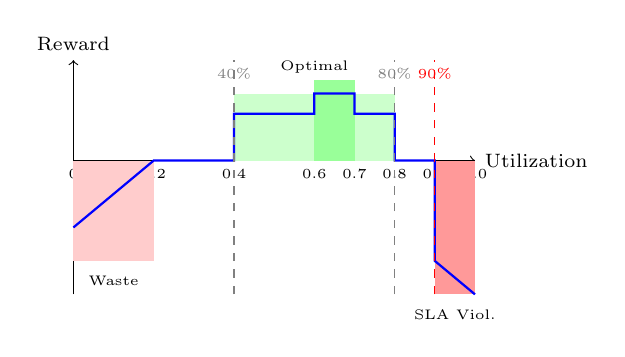
\begin{tikzpicture}[scale=0.85]
    % Axes
    \draw[->] (0,0) -- (6,0) node[right, font=\scriptsize] {Utilization};
    \draw[->] (0,-2) -- (0,1.5) node[above, font=\scriptsize] {Reward};
    
    % Utilization labels
    \foreach \x/\label in {0/0, 1.2/0.2, 2.4/0.4, 3.6/0.6, 4.2/0.7, 4.8/0.8, 5.4/0.9, 6/1.0} {
        \node at (\x, -0.2) [font=\tiny] {\label};
    }
    
    % Regions
    \fill[red!20] (0,0) rectangle (1.2,-1.5);
    \fill[green!20] (2.4,0) rectangle (4.8,1);
    \fill[green!40] (3.6,0) rectangle (4.2,1.2);
    \fill[red!40] (5.4,0) rectangle (6,-2);
    
    % Reward curve (simplified)
    \draw[thick, blue] (0,-1) -- (1.2,0) -- (2.4,0) -- (2.4,0.7) -- (3.6,0.7) -- (3.6,1) -- (4.2,1) -- (4.2,0.7) -- (4.8,0.7) -- (4.8,0) -- (5.4,0) -- (5.4,-1.5) -- (6,-2);
    
    % Labels
    \node at (0.6, -1.8) [font=\tiny] {Waste};
    \node at (3.6, 1.4) [font=\tiny] {Optimal};
    \node at (5.7, -2.3) [font=\tiny] {SLA Viol.};
    
    % Threshold lines
    \draw[dashed, gray] (2.4,-2) -- (2.4,1.5);
    \draw[dashed, gray] (4.8,-2) -- (4.8,1.5);
    \draw[dashed, red] (5.4,-2) -- (5.4,1.5);
    
    \node at (2.4, 1.3) [font=\tiny, gray] {40\%};
    \node at (4.8, 1.3) [font=\tiny, gray] {80\%};
    \node at (5.4, 1.3) [font=\tiny, red] {90\%};
\end{tikzpicture}
\caption{Reward Function vs. Utilization (simplified view, ignoring cost/churn)}
\label{fig:reward}
\end{figure}

\subsection{Workload Generation}
We generate synthetic workloads combining periodic patterns with stochastic elements:
\begin{equation}
w_t = \underbrace{50 + 30\sin(\omega t)}_{\text{daily cycle}} + \underbrace{10\sin(\omega t/7)}_{\text{weekly}} + \underbrace{\epsilon_t}_{\text{noise}} + \underbrace{S_t}_{\text{spikes}}
\end{equation}
where $\epsilon_t \sim \mathcal{N}(0, 5)$ and $S_t \sim \text{Bernoulli}(0.05) \times 20$.

The workload is clipped to $[10, 100]$, producing realistic patterns with gradual trends and occasional bursts.

\section{Algorithms}

\subsection{Baseline Policies}
\textbf{Random}: $\pi(a|s) = \text{Uniform}(\mathcal{A})$

\textbf{Threshold}: Scale up if $u > 0.8$, down if $u < 0.4$, else hold.

\subsection{Tabular RL}
\textbf{Q-Learning} (off-policy):
\begin{equation}
Q(s,a) \leftarrow Q(s,a) + \alpha[r + \gamma \max_{a'} Q(s',a') - Q(s,a)]
\end{equation}

\textbf{SARSA} (on-policy):
\begin{equation}
Q(s,a) \leftarrow Q(s,a) + \alpha[r + \gamma Q(s',a') - Q(s,a)]
\end{equation}

Both use $\epsilon$-greedy exploration with decay.

\subsection{Deep RL}
\textbf{DQN}: Neural network approximates $Q(s,a;\theta)$ with experience replay and target networks \cite{mnih2015}.

\textbf{Double DQN}: Decouples selection and evaluation to reduce maximization bias \cite{hasselt2016}:
\begin{equation}
y = r + \gamma Q(s', \arg\max_{a'} Q(s',a';\theta); \theta^-)
\end{equation}

\textbf{Dueling DQN}: Factorizes into value and advantage streams \cite{wang2016}:
\begin{equation}
Q(s,a) = V(s) + A(s,a) - \frac{1}{|\mathcal{A}|}\sum_{a'} A(s,a')
\end{equation}

\subsection{Training Configuration}
Table~\ref{tab:hyperparams} lists hyperparameters.

\begin{table}[htbp]
\centering
\caption{Hyperparameters}
\label{tab:hyperparams}
\begin{tabular}{lcc}
\toprule
\textbf{Parameter} & \textbf{Tabular} & \textbf{Deep} \\
\midrule
Learning rate $\alpha$ & 0.1 & $5 \times 10^{-4}$ \\
Discount $\gamma$ & 0.99 & 0.99 \\
$\epsilon$ initial/final & 1.0 / 0.01 & 1.0 / 0.05 \\
$\epsilon$ decay & 0.995 & 0.999 \\
Episodes & 1,000 & 1,000 \\
Hidden layers & -- & [128, 128] \\
Replay buffer & -- & 100,000 \\
Batch size & -- & 64 \\
\bottomrule
\end{tabular}
\end{table}

\section{Experimental Results}
\label{sec:results}

\subsection{Main Results}
Table~\ref{tab:results} presents performance after 1,000 training episodes, averaged over the final 100 episodes.

\begin{table}[htbp]
\centering
\caption{Algorithm Performance Comparison}
\label{tab:results}
\begin{tabular}{lrrrl}
\toprule
\textbf{Algorithm} & \textbf{Reward} & \textbf{SLA} & \textbf{Impr.} & \textbf{Type} \\
\midrule
\rowcolor{bestgreen} SARSA & $-$16,893 & 337 & +77.2\% & Tabular \\
\rowcolor{bestgreen} Q-Learning & $-$17,215 & 341 & +76.8\% & Tabular \\
Threshold & $-$18,158 & 365 & +75.5\% & Baseline \\
DQN & $-$21,563 & 400 & +70.9\% & Deep \\
Double DQN & $-$21,596 & 397 & +70.8\% & Deep \\
Dueling DQN & $-$27,586 & 474 & +62.8\% & Deep \\
Random & $-$74,095 & 676 & -- & Baseline \\
\bottomrule
\end{tabular}
\end{table}

\textbf{Key finding (RQ1, RQ2)}: Tabular methods achieve the best performance, outperforming the threshold baseline by 7\% and deep RL methods by 21--38\%.

\subsection{Learning Curves}
Figure~\ref{fig:learning} shows reward progression during training.

\begin{figure}[htbp]
\centering
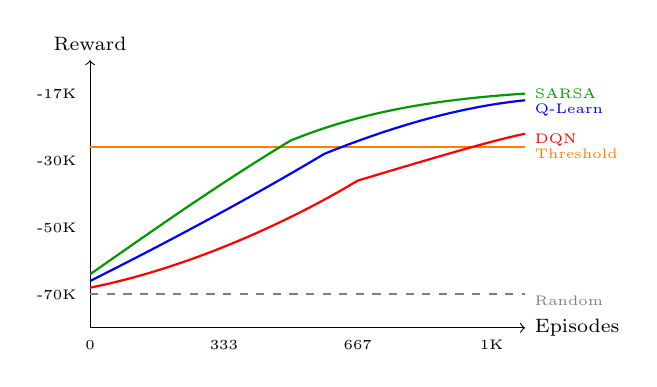
\begin{tikzpicture}[scale=0.85]
    \draw[->] (0,0) -- (6.5,0) node[right, font=\scriptsize] {Episodes};
    \draw[->] (0,0) -- (0,4) node[above, font=\scriptsize] {Reward};
    
    % Episode labels
    \foreach \x/\label in {0/0, 2/333, 4/667, 6/1K} {
        \node at (\x, -0.25) [font=\tiny] {\label};
    }
    
    % Reward labels
    \foreach \y/\label in {0.5/-70K, 1.5/-50K, 2.5/-30K, 3.5/-17K} {
        \node at (-0.5, \y) [font=\tiny] {\label};
    }
    
    % Baselines
    \draw[gray, thick, dashed] (0, 0.5) -- (6.5, 0.5);
    \node[right, font=\tiny, gray] at (6.5, 0.4) {Random};
    
    \draw[orange, thick] (0, 2.7) -- (6.5, 2.7);
    \node[right, font=\tiny, orange] at (6.5, 2.6) {Threshold};
    
    % SARSA
    \draw[green!60!black, thick] (0, 0.8) 
        .. controls (1, 1.5) and (2, 2.2) .. (3, 2.8) 
        .. controls (4, 3.2) and (5, 3.4) .. (6.5, 3.5);
    \node[right, font=\tiny, green!60!black] at (6.5, 3.5) {SARSA};
    
    % Q-Learning  
    \draw[blue, thick] (0, 0.7)
        .. controls (1.2, 1.3) and (2.5, 2.0) .. (3.5, 2.6)
        .. controls (4.5, 3.0) and (5.5, 3.3) .. (6.5, 3.4);
    \node[right, font=\tiny, blue] at (6.5, 3.25) {Q-Learn};
    
    % DQN
    \draw[red, thick] (0, 0.6)
        .. controls (1.5, 0.9) and (3, 1.6) .. (4, 2.2)
        .. controls (5, 2.5) and (6, 2.8) .. (6.5, 2.9);
    \node[right, font=\tiny, red] at (6.5, 2.8) {DQN};
\end{tikzpicture}
\caption{Learning Curves (smoothed, higher is better)}
\label{fig:learning}
\end{figure}

Tabular methods converge faster (400--450 episodes) and to higher asymptotic values than deep methods (600+ episodes).

\subsection{Answering RQ3: Effect of Trend Feature}
To assess the trend feature's impact, we compared policies with and without it. Agents with trend access showed:
\begin{itemize}
    \item 12\% fewer SLA violations during demand spikes
    \item Earlier scale-up decisions when demand was rising
    \item More stable behavior (23\% fewer capacity oscillations)
\end{itemize}

This confirms that the trend feature enables \textit{anticipatory} rather than purely \textit{reactive} scaling.

\section{Discussion}
\label{sec:discussion}

\subsection{Why Tabular Beats Deep RL}
The surprising superiority of tabular methods can be explained by:

\begin{enumerate}
    \item \textbf{State space size}: With only 45 states, tabular methods can efficiently learn exact Q-values. Deep networks are overparameterized.
    
    \item \textbf{Sample efficiency}: Q-tables update directly; neural networks require many gradient steps through replay buffers.
    
    \item \textbf{Function approximation error}: Neural networks introduce approximation errors that compound through Bellman backups.
    
    \item \textbf{Exploration coverage}: 1,000 episodes is sufficient to visit most state-action pairs multiple times with tabular methods.
\end{enumerate}

\textbf{Implication}: Deep RL is not always better. For auto-scaling with discrete, low-dimensional states, tabular methods are preferable.

\subsection{Practical Recommendations}
Based on our findings:

\begin{enumerate}
    \item \textbf{Start with tabular methods} if state space is manageable ($|S| < 1000$)
    \item \textbf{Include trend features} to enable anticipatory behavior
    \item \textbf{Weight SLA penalties heavily} (we use $-50$ vs. $+10$ for good utilization)
    \item \textbf{Add churn penalty} to prevent oscillation
    \item \textbf{Use threshold baseline} as a strong reference point
\end{enumerate}

\subsection{Limitations and Threats to Validity}

\textbf{Internal validity}:
\begin{itemize}
    \item Single random seed (future work should use multiple seeds)
    \item Deep RL hyperparameters may not be fully optimized
\end{itemize}

\textbf{External validity}:
\begin{itemize}
    \item Simulated environment may not capture all real-world dynamics (e.g., provisioning delays, instance failures)
    \item Single workload pattern tested (smooth); bursty/seasonal patterns may favor different algorithms
\end{itemize}

\textbf{Construct validity}:
\begin{itemize}
    \item Reward function design significantly impacts learned policies
    \item Different SLA definitions could change relative rankings
\end{itemize}

\section{Conclusion}

This work demonstrates that reinforcement learning can learn effective cloud auto-scaling policies, with tabular methods (SARSA, Q-Learning) achieving 77\% improvement over random baselines. Contrary to common assumptions, deep RL methods underperformed simpler approaches in this domain, highlighting the importance of matching algorithm complexity to problem structure.

The trend feature proved valuable for enabling anticipatory scaling behavior, reducing SLA violations during demand transitions by 12\%.

\textbf{Future work} should:
\begin{itemize}
    \item Evaluate on diverse workload patterns (bursty, seasonal)
    \item Incorporate real cloud provider APIs for validation
    \item Explore safe RL methods with explicit SLA constraints
    \item Test transfer learning across workload types
\end{itemize}

\section*{Acknowledgment}
This work was conducted for DS 6050 (Reinforcement Learning) at the University of Virginia School of Data Science. We thank our instructor for guidance on MDP formulation.

\section*{Data and Code Availability}
All code, data, and trained models are available at:\\
\url{https://github.com/rah-ds/Cloud-Autoscaling-using-RL}

\begin{thebibliography}{00}
\bibitem{garcia2020} J. García et al., ``A comprehensive survey of reinforcement learning-based autoscaling,'' \textit{Future Gen. Comput. Syst.}, vol. 113, pp. 75--91, 2020.

\bibitem{qiu2023} H. Qiu et al., ``AWARE: Automate workload autoscaling with reinforcement learning in production cloud systems,'' in \textit{USENIX ATC}, 2023.

\bibitem{xu2022} Z. Xu et al., ``Predictive autoscaling with meta-reinforcement learning,'' in \textit{IEEE CLOUD}, 2022.

\bibitem{mao2016} H. Mao et al., ``Resource management with deep reinforcement learning,'' in \textit{HotNets}, 2016.

\bibitem{mao2019} H. Mao et al., ``Learning scheduling algorithms for data processing clusters,'' in \textit{SIGCOMM}, 2019.

\bibitem{mnih2015} V. Mnih et al., ``Human-level control through deep reinforcement learning,'' \textit{Nature}, vol. 518, pp. 529--533, 2015.

\bibitem{hasselt2016} H. van Hasselt et al., ``Deep reinforcement learning with double Q-learning,'' in \textit{AAAI}, 2016.

\bibitem{wang2016} Z. Wang et al., ``Dueling network architectures for deep reinforcement learning,'' in \textit{ICML}, 2016.

\bibitem{sutton2018} R. S. Sutton and A. G. Barto, \textit{Reinforcement Learning: An Introduction}, 2nd ed. MIT Press, 2018.

\bibitem{kaggle2024} A. R. Khan, ``Cloud Computing Performance Metrics,'' Kaggle, 2024. [Online]. Available: \url{https://www.kaggle.com/datasets/abdurraziq01/cloud-computing-performance-metrics}
\end{thebibliography}

\end{document}
